% !TEX root = ../Survey.tex
\section{Bounded cases}\label{section:bounded-cases}
We describe the new results mentioned in table ~\ref{Table2}.
%\paragraph{Routing}
\paragraph{Ancestry}
	\begin{thm} \label{thm:cat-anc}
		 $Caterpillars(n)$ have an ancestry  labeling scheme of $ \log n + \Theta(1)$
	\end{thm}
		\begin{proof}
			 Note that in contrast to general case,  only internal vertices can be mutual ancestors.
	 		Let $I_1 \dots I_k$ be the internal vertices of the rooted caterpillar $T = (V,E)$, for each  $1 \leq i \leq k$ we mark the $k_i$ leaves of $I_i$ as $L_i^1 \dots L_i^{k_i}$.
			Let $r  \in V$ be the root of $T$. 
			The encoder assigns  each node  a number in the range $[1 \dots n]$ using a BFS scan on $T$ from $r$.
			The connected internal node is last in the scan and receives the number $k_1 +1$, and the labeling continues recursively.
			We mark internal vertices by a prefix $0$ to the label, and $1$  for a leaf.
			
			For query $Ancestor(u,v)$, the decoder can safely reject if $u$ and $v$ are leaves.
			Otherwise, the query would return true if and only if $u<v$.
		 \end{proof}
 \paragraph{Distance}
	 \begin{thm} \label{thm:cat-dist}
	 $Caterpillars(n)$ have a distance labeling scheme of $2 \log n$
	 \end{thm}
	 
	 \begin{proof}
	 Let $I_1 \dots I_k$ be the internal vertices of the caterpillar $T$, for each  $1 \leq i \leq k$ we mark the $k_i$ leaves of $I_i$ as $L_i^1 \dots L_i^{k_i}$.
	 The encoder assigns $I_i$ the label $\tuple{i,0}$ and its leaves $L_i^1 \dots L_i^{k_i}$ the labels $\tuple{i,1} \dots \tuple{i,k}$ in according.
	 Assume that $a \geq c$.
	 The decoder acts on query $Distance(\tuple{a,b},\tuple{c,d})$ as follows:
	 	\begin{enumerate}
		\item $b=d=0$ : return $a-c$
		\item $ b\neq 0 ,d \neq 0$ : return $a-c+2$ if $ a \neq c$ and $0$ otherwise.
		\item $ b = 0 ,d \neq 0$ or  $ b  \neq 0,d = 0$  : return $a-c+1$
	 	\end{enumerate}
		Since $1 \leq i,k_i \leq n$ we conclude that the latter can be decoded using (exactly) $ 2 \log n$ bits.
		Moreover, for $Caterpillars(n,\Delta)$, $k_i \leq \Delta$, and for $Caterpillars(n,\delta)$, $i \leq \Delta$.
		Thus, for both cases  only $  \log n + \log \Delta $  are required.
 	 \end{proof}
	 
	 If $T$ is an edge  weighted with maximum edge weight $2^M$ we assign  for $I_i$ with weight $w(I_i)$ the label $\tuple{\sum_{j=1}^{i} w(I_j) ,0,0}$ 
	 
	 The leaves $L_i^1 \dots L_i^{k_i}$ are assigned the labels
	 
	  $\tuple{\sum_{j=1}^{i} w(I_j) , w(L_i^1)  ,1} \dots \tuple{\sum_{j=1}^{i} w(I_j) , w(L_i^{k+1})  ,k+1} $ in according.
	  
	   Assume that $a \geq d$.
	 The decoder now  acts on query $Distance(\tuple{a,b,c},\tuple{d,e,f})$ as follows:
	 	\begin{enumerate}
		\item $c=f=0$ : return $a-d$
		\item $ c\neq 0 ,f \neq 0$ : if $\tuple{a,b,c} \neq \tuple{d,e,f}$  return $a-d+b+e$, otherwise  $0$.
		\item $ c = 0 ,f  \neq 0$ : return $a-d+e$
		\item $ c \neq  0 ,f  = 0$ : return $a-d+b$
	 	\end{enumerate}
		
		
	 \begin{corollary}\label{Cor:lowerbounds}
	 \hfill
	 \begin{itemize}
	 	\item Edge weighted $Caterpillars(n,2^M)$  have a distance labeling scheme of $2 \log n + 2M$
		\item  Edge weighted  $Caterpillars(n,\Delta,2^M)$   have a distance labeling scheme of $ \log n  + \log \Delta + 2M$
	\end{itemize}
	 \end{corollary}
%
%\paragraph{Center}
%
%	 \begin{thm} \label{thm:cat-dist}
%	 $Caterpillars(n)$ have a center  labeling scheme of $2 \log n$
%	 \end{thm}
%	 
%	 \begin{proof}
%	 
%	 \end{proof}

\paragraph{The implications of Alstrup's lower bounds on the limited variants}
The limits attained by Alstrup \cite{Alstrup05} applies directly for ancestry in the bounded depth and degree cases. The sibling bound applies  for caterpillars,  and bounded  depth trees.
As seen in Figure~\ref{fig:loubou}, the lower bound for siblings is defined for $\delta =3$. Moreover, each tree of the $\log n$ trees in the family can be transformed  to a caterpillar in the following manner.
Denote the set of nodes neighboring to the root by $v_1 \dots v_i$.  We remove the root $r$ and for each  $1 \leq  j < i$  we replace each edge $(r,v_j)$ with $(v_j,v_{j+1})$ .
The transformed  family of caterpillars  maintains  the  lower bound for sibling relation.

We can thus conclude:

	\begin{corollary}
	\hfill
	 	\begin{itemize}
		\item  Any sibling labeling scheme for $Caterpillars(n)$  must have a labeling scheme of at least  $ \log n +O(\log \log n)$ bits.
		\item	Any sibling labeling scheme for $Caterpillars(n,\delta)$ ($\delta \geq 2$)  must have a labeling scheme of  at least $ \log n +O(\log \log n)$ bits.
		\end{itemize}
	\end{corollary}

\begin{figure}
\centering
\makebox[\textwidth][c]{
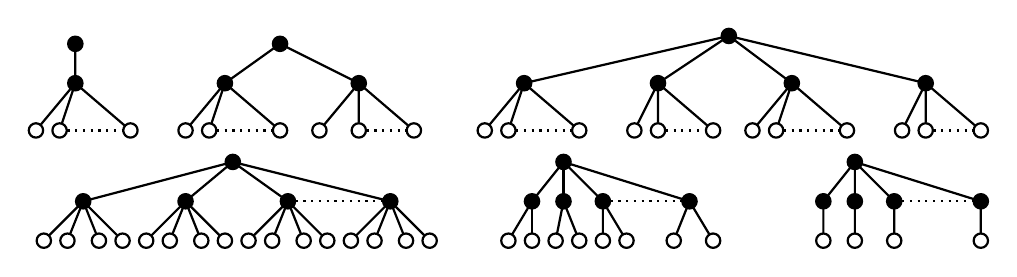
\begin{tikzpicture}[thick,scale=0.4, every node/.style={scale=0.55}]

\tikzstyle{Node}=[circle,fill=White,draw=Black]

\tikzstyle{NiceNode}=[circle,fill=White,draw=Black,scale = 1,
font=\small]

\tikzstyle{Edge}=[]

\tikzstyle{NiceEdge}=[dotted]

\tikzstyle{ControlNodes} = [circle,fill=Black,draw=Black]

\tikzstyle{none}=[inner sep=0pt]
		\node [style=ControlNodes] (0) at (-9, 1.5) {};
		\node [style=NiceNode] (1) at (-10.25, 0) {};
		\node [style=NiceNode] (2) at (-9.5, 0) {};
		\node [style=NiceNode] (3) at (-7.25, 0) {};
		\node [style=ControlNodes] (4) at (-4.75, 1.5) {};
		\node [style=NiceNode] (5) at (-6, 0) {};
		\node [style=NiceNode] (6) at (-3, 0) {};
		\node [style=NiceNode] (7) at (-4.75, 0) {};
		\node [style=ControlNodes] (8) at (-7.25, 2.75) {};
		\node [style=ControlNodes] (9) at (7, 3) {};
		\node [style=ControlNodes] (10) at (4.75, 1.5) {};
		\node [style=NiceNode] (11) at (-0.75, 0) {};
		\node [style=NiceNode] (12) at (4.75, 0) {};
		\node [style=NiceNode] (13) at (2.25, 0) {};
		\node [style=ControlNodes] (14) at (0.5, 1.5) {};
		\node [style=NiceNode] (15) at (4, 0) {};
		\node [style=NiceNode] (16) at (6.5, 0) {};
		\node [style=NiceNode] (17) at (0, 0) {};
		\node [style=NiceNode] (18) at (8.5, 0) {};
		\node [style=ControlNodes] (19) at (9, 1.5) {};
		\node [style=NiceNode] (20) at (7.75, 0) {};
		\node [style=NiceNode] (21) at (13.25, 0) {};
		\node [style=ControlNodes] (22) at (13.25, 1.5) {};
		\node [style=NiceNode] (23) at (15, 0) {};
		\node [style=NiceNode] (24) at (10.75, 0) {};
		\node [style=NiceNode] (25) at (12.5, 0) {};
		\node [style=NiceNode] (26) at (-15, 0) {};
		\node [style=NiceNode] (27) at (-12, 0) {};
		\node [style=ControlNodes] (28) at (-13.75, 1.5) {};
		\node [style=NiceNode] (29) at (-14.25, 0) {};
		\node [style=ControlNodes] (30) at (-13.75, 2.75) {};
		\node [style=ControlNodes] (31) at (1.75, -1) {};
		\node [style=NiceNode] (32) at (5.25, -3.5) {};
		\node [style=ControlNodes] (33) at (3, -2.25) {};
		\node [style=NiceNode] (34) at (3.75, -3.5) {};
		\node [style=NiceNode] (35) at (1.5, -3.5) {};
		\node [style=NiceNode] (36) at (6.5, -3.5) {};
		\node [style=ControlNodes] (37) at (5.75, -2.25) {};
		\node [style=NiceNode] (38) at (0.75, -3.5) {};
		\node [style=NiceNode] (39) at (0, -3.5) {};
		\node [style=ControlNodes] (40) at (1.75, -2.25) {};
		\node [style=ControlNodes] (41) at (0.75, -2.25) {};
		\node [style=NiceNode] (42) at (3, -3.5) {};
		\node [style=NiceNode] (43) at (2.25, -3.5) {};
		\node [style=NiceNode] (44) at (15, -3.5) {};
		\node [style=ControlNodes] (45) at (11, -1) {};
		\node [style=ControlNodes] (46) at (15, -2.25) {};
		\node [style=NiceNode] (47) at (11, -3.5) {};
		\node [style=ControlNodes] (48) at (10, -2.25) {};
		\node [style=ControlNodes] (49) at (11, -2.25) {};
		\node [style=ControlNodes] (50) at (12.25, -2.25) {};
		\node [style=NiceNode] (51) at (12.25, -3.5) {};
		\node [style=NiceNode] (52) at (10, -3.5) {};
		\node [style=NiceNode] (53) at (-14.75, -3.5) {};
		\node [style=ControlNodes] (54) at (-13.5, -2.25) {};
		\node [style=ControlNodes] (55) at (-8.75, -1) {};
		\node [style=NiceNode] (56) at (-13, -3.5) {};
		\node [style=NiceNode] (57) at (-14, -3.5) {};
		\node [style=NiceNode] (58) at (-12.25, -3.5) {};
		\node [style=NiceNode] (59) at (-10.75, -3.5) {};
		\node [style=NiceNode] (60) at (-11.5, -3.5) {};
		\node [style=ControlNodes] (61) at (-10.25, -2.25) {};
		\node [style=NiceNode] (62) at (-9, -3.5) {};
		\node [style=NiceNode] (63) at (-9.75, -3.5) {};
		\node [style=NiceNode] (64) at (-5.75, -3.5) {};
		\node [style=ControlNodes] (65) at (-7, -2.25) {};
		\node [style=NiceNode] (66) at (-8.25, -3.5) {};
		\node [style=NiceNode] (67) at (-7.5, -3.5) {};
		\node [style=NiceNode] (68) at (-6.5, -3.5) {};
		\node [style=NiceNode] (69) at (-2.5, -3.5) {};
		\node [style=ControlNodes] (70) at (-3.75, -2.25) {};
		\node [style=NiceNode] (71) at (-5, -3.5) {};
		\node [style=NiceNode] (72) at (-4.25, -3.5) {};
		\node [style=NiceNode] (73) at (-3.25, -3.5) {};
		\draw (0) to (1);
		\draw (0) to (2);
		\draw (0) to (3);
		\draw [style=NiceEdge] (2) to (3);
		\draw (4) to (5);
		\draw (4) to (7);
		\draw (4) to (6);
		\draw [style=NiceEdge] (7) to (6);
		\draw (0) to (8);
		\draw (8) to (4);
		\draw (14) to (11);
		\draw (14) to (17);
		\draw (14) to (13);
		\draw [style=NiceEdge] (17) to (13);
		\draw (10) to (15);
		\draw (10) to (12);
		\draw (10) to (16);
		\draw [style=NiceEdge] (12) to (16);
		\draw (14) to (9);
		\draw (9) to (10);
		\draw (19) to (20);
		\draw (19) to (18);
		\draw (19) to (24);
		\draw [style=NiceEdge] (18) to (24);
		\draw (22) to (25);
		\draw (22) to (21);
		\draw (22) to (23);
		\draw [style=NiceEdge] (21) to (23);
		\draw [style=Edge] (9) to (19);
		\draw [style=Edge] (9) to (22);
		\draw (28) to (26);
		\draw (28) to (29);
		\draw (28) to (27);
		\draw [style=NiceEdge] (29) to (27);
		\draw (28) to (30);
		\draw (41) to (39);
		\draw (41) to (38);
		\draw (40) to (35);
		\draw (40) to (43);
		\draw (41) to (31);
		\draw (31) to (40);
		\draw (33) to (42);
		\draw (33) to (34);
		\draw (37) to (32);
		\draw (37) to (36);
		\draw [style=Edge] (31) to (33);
		\draw [style=Edge] (31) to (37);
		\draw [style=NiceEdge] (33) to (37);
		\draw (48) to (52);
		\draw (49) to (47);
		\draw (48) to (45);
		\draw (45) to (49);
		\draw (50) to (51);
		\draw (46) to (44);
		\draw [style=Edge] (45) to (50);
		\draw [style=Edge] (45) to (46);
		\draw [style=NiceEdge] (50) to (46);
		\draw (54) to (53);
		\draw (54) to (56);
		\draw (54) to (55);
		\draw [style=Edge] (54) to (57);
		\draw [style=Edge] (54) to (58);
		\draw (61) to (60);
		\draw (61) to (63);
		\draw [style=Edge] (61) to (59);
		\draw [style=Edge] (61) to (62);
		\draw (65) to (66);
		\draw (65) to (68);
		\draw [style=Edge] (65) to (67);
		\draw [style=Edge] (65) to (64);
		\draw (70) to (71);
		\draw (70) to (73);
		\draw [style=Edge] (70) to (72);
		\draw [style=Edge] (70) to (69);
		\draw [style=Edge] (55) to (61);
		\draw [style=Edge] (55) to (65);
		\draw [style=Edge] (55) to (70);
		\draw [style=NiceEdge] (65) to (70);
		
\end{tikzpicture}
}
\caption{The 3 first (First line)  and 3 last  (Second line)  members of the  family of trees introduced for the siblings lower bounds} \label{fig:loubou}
\end{figure}

